\documentclass[conference]{IEEEtran}
\IEEEoverridecommandlockouts
% The preceding line is only needed to identify funding in the first footnote. If that is unneeded, please comment it out.
\usepackage{cite}
\usepackage{amsmath,amssymb,amsfonts}
\usepackage{algorithmic}
\usepackage{graphicx}
\usepackage{textcomp}
\usepackage{xcolor}
\usepackage{hyperref}

\interdisplaylinepenalty=2500
\def\BibTeX{{\rm B\kern-.05em{\sc i\kern-.025em b}\kern-.08em
    T\kern-.1667em\lower.7ex\hbox{E}\kern-.125emX}}
\begin{document}

\title{PyIF: A Fast and Light Weight Implementation to Estimate Bivariate Transfer Entropy for Big Data
%\thanks{Identify applicable funding agency here. If none, delete this.}
}

\author{\IEEEauthorblockN{Kelechi M. Ikegwu}
\IEEEauthorblockA{IIlinois Informatics Institute  \\
\textit{University of Illinois at Urbana-Champaign}\\
Urbana, IL USA \\
ikegwu2@illinois.edu}
\and
\IEEEauthorblockN{Jacob Trauger}
\IEEEauthorblockA{Department of Computer Science \\
\textit{University of Illinois at Urbana-Champaign}\\
Urbana, IL, USA \\
jtt2@illinois.edu}
\and
\IEEEauthorblockN{Jeff McMullin}
\IEEEauthorblockA{Department of Accounting \\
\textit{Indiana University}\\
Bloomington, IN, USA  \\
jemcmull@indiana.edu}
\and
\IEEEauthorblockN{Robert J. Brunner}
\IEEEauthorblockA{Department of Accountancy  \\
\textit{University of Illinois at Urbana-Champaign}\\
Urbana, IL, USA \\
bigdog@illinois.edu}
}

\maketitle

\begin{abstract}
Transfer entropy is an information measure that quantifies information flow between processes evolving in time. Transfer entropy has a plethora of potential applications in financial markets, canonical systems, neuroscience, and social media. We offer a fast open source Python implementation called PyIF that estimates Transfer Entropy with Kraskov's method. PyIF utilizes KD-Trees, multiple processes by parallelizing queries on said KD-Trees, and can be used with CUDA compatible GPUs to significantly reduce the wall time for estimating transfer entropy. We find from our analyses that PyIF's GPU implementation is up to 1072 times faster (and it's CPU implementation is up 181 times faster) than existing implementations to estimate transfer entropy on large data and scales better than existing implementations.
\end{abstract}

\begin{IEEEkeywords}
Transfer Entropy, Parallel Processing
\end{IEEEkeywords}

\section{Introduction}

Information theory provides a framework for studying the quantification, storage, and communication of information \cite{InfoTheoryApplications}.  This theory defines entropy as the amount of uncertainty or disorder in a random process. Mutual Information is another measure in this theory which quantifies the amount of information shared across random variables. While similar to mutual information, transfer entropy (TE) also considers the dynamics of information and how these dynamics evolves in time.\cite{IntroToTransferEntropy}. Put simply, TE quantifies the reduction in uncertainty in one random process from knowing past realizations of another random process. This is a particularly useful property of TE as many real-world phenomena, from stock market prices to neural signals, are dynamic processes evolving in time. TE is also an asymmetric measure of information transfer. Ergo, TE computed from process \(A\) to process \(B\) may yield a different result than TE computed from \(B\) to \(A\). The information theoretic framework and these measures have led to a variety of applications in different research areas \cite{InfoTheoryApplications}, \cite{TEBook}.


\subsection{Applications of Transfer Entropy}

TE is particularly useful for detecting information transfer in financial markets \cite{TEBook}. Marschinski and Kantz used TE to perform index-to-index analysis with the Dow Jones Share Market (DJIA) and the Frankfurt Stock index (DAX) \cite{FinAppTE} and document the extent to which one index drives the behavior of the other. Following Marschinski and Kantz, other researchers apply TE to examine related research questions about financial markets. These include measuring TE from market indexes, such as S\&P 500 or the DJIA, to individual equities as well as between individual equities \cite{TEBook}.

Network Inference is another application area of TE. An objective of network inference is to infer a network by indentifying relationships between individual processes in the data. Computational neuroscience, financial market analysis, gene regulatory networks, social media, and multi-agent systems are areas where TE has been used to model networks. Early approaches that used TE for  network inference either measure pairwise TE between all pairs of variables in a network or threshold the TE values to select connections between nodes in a network \cite{NetworkTEApp1}, \cite{NetworkTEApp2}, and \cite{NetworkTEApp3}. Recent approaches have used statistical significance tests of pairwise TE to determine whether links exist \cite{NetworkTEApp4} and \cite{NetworkTEApp5}. \cite{TEBook} offers more examples of TE applications.

\subsection{Outline}
In the next section we formally define TE. The following section discusses TE estimation methods. We then discuss our our proposed implementation called PyIF to estimate bivariate TE. Next, we describe a comparative analysis between PyIF and existing implementations that estimate bivariate TE. Lastly, we conclude the paper with a discussion and future work.


\section{Definition of Transfer Entropy}

In 2000, Schreiber \cite{IntroToTransferEntropy} discovered TE and coined the name ``transfer entropy," although Milian Palus \cite{IntroToTransferEntropy2} also independently discovered the concept as well. Let the function \(I\) represent mutual information between two probability distributions. Lagged mutual information \(I(X_t : Y_{t-k})\) can be used as a time-asymmetric measure of information transfer from \(Y\) to \(X\) where \(X\) and \(Y\) are both random processes, \(k\) is a lag period, and \(t\) is the current time period. However, lagged mutual information is unsatisfactory as it does not account for a shared history between the processes \(X\) and \(Y\) \cite{MIdiffTE}.

TE considers the shared history between two processes via conditional mutual information. Specifically, TE conditions on the past of \(X_t\) to remove any redundant or shared information between \(X_t\) and its past. This also removes any information in the process \(Y\) about \(X\) at time \(t\) that is in the past of \(X\) \cite{b359}. Transfer entropy \(T\) (where the transfer of information occurs from \(Y\) to \(X\)) can be defined as:
\begin{equation}
T_{Y \rightarrow X} (t) \equiv I(X_t: Y_{t-k} |  X_{t-k}).
\end{equation}

Kraskov \cite{kraskovEstimator} shows that transfer entropy can be expressed as the difference between two conditional mutual information computations: \begin{equation} T_{Y \rightarrow X}(t) = I(X_t | X_{t-k}, Y_{t-k}) -  I(X_t | X_{t-k})  \end{equation} .

The intuition of this definition is that TE measures the amount of information in \(Y_{t-k}\) about \(X_t\) after  considering the information in \(X_{t-k}\) about \(X_t\). Put differently, TE quantifies the reduction in uncertainty about \(X_t\) from knowing \(Y_{t-k}\) after considering the reduction in uncertainty about \(X_t\) from knowing \(X_{t-k}\).

\section{Estimating Transfer Entropy}

There are many techniques for estimating mutual information. Khan et al. explored the utility of different methods for mutual information estimation \cite{EstimatingTE} and many of the methods they considered are applicable to estimate TE.

\subsection{Kernel Density Estimator}
Kernel Density Estimators can be used to estimate TE \cite{KDE}. For a bivariate dataset of size n with variables X and Y, Mutual Information can be estimated as:

\begin{equation}\hat{I}(X,Y) = \frac{1}{n} \sum_{i=1}^n ln \frac{\hat{p}_{XY}(x_i, y_j)  } {\hat{p}_X(x_i) \hat{p}_Y(y_i)}  \end{equation}

\noindent where \(\hat{p}_X(x_i)\) and \( \hat{p}_Y(y_i)\) are the estimated marginal probability density functions and  \(\hat{p}_{XY}(x_i, y_j)\) is the joint estimated probability density function. For a multivariate dataset containing: \(x_1, x_2, ..., x_n\) where each \(x\) is in a d-dimensional space, the multivariate kernel density estimator with kernel \(K\) is defined by:

\begin{equation}\hat{p}(x) = \frac{1}{nh^d} \sum_i=1^n K(\frac{x-x_i}{h}  )\end{equation}

\noindent where \(h\) is the smoothing parameter, and in this case, \(K\) is a standard multivariate normal kernel defined by \(K(x)=(2\pi)^{-d/2} e^{\frac{x^Tx}{2} } \). Moon et al. outlined a procedure to estimate Mutual Information using marginal and joint probabilities with Kernel Density Estimators \cite{KDE}.

\subsection{Kraskov Estimator}

Transfer Entropy can be estimated using k-nearest neighbors \cite{kraskovEstimator}. Note that entropy can be estimated with:

\begin{equation}\hat{H}(X) = - \frac{1}{n} \sum^n_{i=1} ln \hat{p}(x_i) \end{equation}

Kraskov et al. expanded this definition to estimate entropy to:

\setlength{\arraycolsep}{0.0em}
\begin{eqnarray}
\hat{H}(X) = - \frac{1}{n} \sum^n_{i=1} \psi(n_x(i)) - \frac{1}{k} + \psi(n) + ln (c_{d_x}) + \nonumber\\
 \frac{d_x}{n} \sum^n_{i=1} ln (\epsilon(i))
\end{eqnarray}
\setlength{\arraycolsep}{1pt}

%\begin{equation} \hat{H}(X) = - \frac{1}{n} \sum^n_{i=1} \psi(n_x(i)) - \frac{1}{k} + \psi(n) + ln (c_{d_x}) + \frac{d_x}{n} \sum^n_{i=1} ln (\epsilon(i)) \end{equation},
\noindent where n are the number of data points, k are the nearest neighbors, \(d_x\) is the dimension of x, and \(c_{d_x}\) is the volume of the \(d_x\)-dimensional unit ball. For two random variables X and Y, let \( \frac{\epsilon(i)}{2} \) be the distance between (\(x_i,y_i\)) and it's k\textsuperscript{th} neighbor be denoted by (\(kx_i,ky_i\)). Let \(\frac{\epsilon_x(i)}{2}\) and  \(\frac{\epsilon_y(i)}{2}\) be defined as \( ||x_i-kx_i ||\) and \( ||y_i-y_i || \) respectively. \(n_x(i)\) is the number of points \(x_j\) such that \(||x_i - x_j  || \leq \epsilon_x(i)/2\), \(\psi(x)\) is the digamma function where

\begin{equation}\psi(x) = \Gamma(x)^-1 d\Gamma(x) / dx \end{equation}
and  \(\Gamma(x)\) is the ordinary gamma function. Lastly \(\psi(1) = -C\) where \(C=0.5772156649\) and is the Euler-Mascheroni constant. To estimate the entropy for the random variable Y, \(Y\) can be substituted into \(\hat{H}(X)\).

Joint entropy between X and Y can then be estimated as:
\setlength{\arraycolsep}{0.0em}
\begin{eqnarray}
\hat{H}(X,Y) = - \psi(k) - \frac{1}{k} + \psi(n) + ln(c_{d_x} c_{d_y})  +  \nonumber\\
\frac{d_x + d_y}{n} \sum^n_i ln(\epsilon(i)
\end{eqnarray}
\setlength{\arraycolsep}{1pt}

%\begin{equation}\hat{H}(X,Y) = - \psi(k) - \frac{1}{k} + \psi(n) + ln(c_{d_x} c_{d_y})  + \frac{d_x + d_y}{n} \sum^n_i ln(\epsilon(i))\end{equation}

\noindent where \(d_y\) is the dimension of \(y\), and \(c_{d_y}\) is the column of the \(d_y\)-dimensional unit ball. Using \(\hat{H}(X), \hat{H}(Y),\) and \(\hat{H(X,Y)}\) mutual information can be estimated as:

\begin{equation}
\label{KraskovEquation}
\hat{I}(X,Y) = \psi(k) - \frac{1}{k} - \frac{1}{n}  \sum_{i=1}^n [\psi(n_x(i)) + \psi(n_y(i))] + \psi(n)
\end{equation}

\noindent where \(n_y(i)\) is the number of points \(y_j\) such that \(|| y_i - y_j || \leq \frac{\epsilon_y(i)}{2} \). This method has been referred to as the Kraskov estimator in literature.

\subsection{Additional Estimators}
Khan et al. also explored the utility of Edgeworth approximation of differential entropy to calculate Mutual Information and adaptive partitioning of the XY plane to estimate the joint probability density, which can be used to estimate mutual information. Ultimately Khan et al. found that a KDE estimator and Kraskov estimator outperform  other methods  with respect to their ability to capture the dependence structure of random processes. Currently our software supports estimating bivariate TE using the Kraskov estimator with plans to add other estimators in the future.

\section{PyIF}

Our proposed software implementation PyIF \footnote{PyIF can freely be downloaded from: \url{https://github.com/lcdm-uiuc/PyIF}} is an open source implementation. PyIF currently only supports using the Kraskov estimator to estimate TE. PyIF utilizes recent advancements in hardware to parallelize \& optimize operations across CPUs and Cuda compatible GPUs \cite{CUDA} and CPUs. In particular we focus our efforts on the parallelization \& optimization across operations to obtain \(n_x\)  \& \(n_y\) in Eq. \ref{KraskovEquation} faster.

PyIF is a python only implementation which utilizes 5 well-known and actively supported python libraries: SciPy \cite{scipy}, NumPy \cite{numpy}, scikit-learn \cite{sklearn}, nose \cite{nose}, and numba \cite{numba}.  SciPy is an open source Python library used for a variety of STEM applications. NumPy  is a part of SciPy's ecosystem and is an open source package that provides convenient ways to perform matrix manipulations and useful linear algebra capabilities. The library scikit-learn is a popular open source library for machine learning and nose is another open source library that is useful for testing code to ensure that it will produce the correct outcome. Lastly, numba is a python compiler that can compile Python code for execution on multicore CPUs and CUDA-capable GPUs.

PyIF's  interface only requires you to supply \(X\) and \(Y\), two numpy arrays with \(N\)x1 dimensions. Optional arguments can be passed in such as \(k\) which controls the number of neighbors used in KD-tree queries, \(embedding\) which controls how many lagged periods are used to estimate transfer entropy and a boolean argument \(GPU\) can be used to specify if you want to use a CUDA compatible GPU. Lastly another boolean argument \(safetyCheck\) can be used to check for duplicates rows in your dataset. This boolean argument is there to help prevent a more subtle error that can occur when multiple data points in a bivariate dataset have identical coordinates. This essentially can lead to several points that have an identical distance to a query point which violates assumptions of the Kraskov estimator. A solution that is used in practice and that we recommend is to add a small amount of noise to your dataset to avoid this error.

\section{Comparative Analysis}

We compare PyIF's ability to estimate Transfer Entropy against existing implementations with respect to computational performance. We present all of the data and code used to estimate TE for all implementations \footnote{The data and code can freely be downloaded from: \url{https://github.com/lcdm-uiuc/Publications/2020\_Ikegwu\_Traguer\_McMullin\_Brunner}}. Each implementation in this comparative analysis estimates TE on four simulated bivariate datasets of different sizes. The estimated TE values are roughly the same for each implementation and we forgo comparing the actual values since this is random simulated data. We make the assumption that there is relatively little to no information transfer between the random processes. We run each of the implementations (excluding Transfer Entropy Toolbox)  on nano, a cluster of eight SuperMicro servers with Intel Haswell/Broadwell CPUs and NVIDIA Tesla P100/V100 GPUs hosted by the National Center of Super Computing Applications at the University of Illinois at Urbana-Champaign. We used one node which contains two E5-2620 v3 Intel Xeon CPU's and 2 NVIDIA P100 GPUs with 3584 cores.  We refer to this analysis as Analysis 1.

We conduct the same analysis on different hardware to compare PyIF to Transfer Entropy toolbox because of MATLAB licensing issues with the National Center of Super Computing Applications. We use an Engineering Workstation with an Intel Xeon Processor E5-2680 v4  hosted by Engineering IT shared services at the University of Illinois at Urbana-Champaign. We use a single CPU core and up to 16GB of RAM to estimate TE with Transfer Entropy toolbox and PyIF. This workstation does not offer CUDA compatiable GPUs to use for either PyIF or Transfer Entropy Toolbox so we forgo comparing the GPU implementations. This workstation has a CPU time limit of 60 minutes meaning that if any process uses 100\% of a CPU core for more than 60 minutes the process is terminated. We refer to this analysis as Analysis 2.

\subsection{IDTxl}
The first implementation is the Information Dynamics Toolkit xl (IDTxl). IDTxl is an open source Python toolbox for network inference \cite{IDTxl}. Currently IDTxl relies on NumPy, SciPy, CFFI (which is another open source library that provides a C interface for Python code), H5py which is a Python package that is used to interface with HDF5 binary data format, JPype which is a Python module that provides a Java interface for Python code, and Java jdk which is a developer kit to develop Java applications and applets. IDTxl has additional functionaility besides estimating TE however we only use IDTxl's capability to estimate TE on a bivariate dataset.


\subsection{TransEnt}
TransEnt is a R package that estimates transfer entropy \cite{TransEnt}. Currently TransEnt relies on Rcpp which acts as a interface to C++ from R. TransEnt also relies on  a C++ library called Appromixate Nearest Neigbors (ANN) \cite{ANN} which performs exact and approximate nearest neighbor searches. Currently the package has been removed from CRAN, however this software can be used and installed from \cite{TransEnt}'s github repo \footnote{\cite{TransEnt} Github Repo: \url{https://github.com/Healthcast/TransEnt}}.

\subsection{RTransferEntropy}
RTransferEntropy is a R package that estimates transfer entropy between two time series \cite{RTransferEntropy}. Currently the RTransferEntropy package relies on Rcpp, and the future package which supports performing computations in parallel to decrease the wall time. We include both the parallel implementation of RTransferEntropy and the default implementation for completeness in the results.

\subsection{Transfer Entropy Toolbox}

Transfer Entropy Toolbox  is an open source MATLAB toolbox for transfer entropy estimation \cite{TransferEntropyToolbox}. This code's dependencies include: the Statistics \& Machine Learning toolbox which provides functions to analyze and model data; the FieldTrip toolbox which is used for EEG, iEEG, MEG, and NIRS analysis; the parallel computing toolbox that performs parallel computations of multicore CPUs and GPUs; the signal processing toolbox that provides functions to analyze, preprocess, and extract features from sampled signals; the TSTOOL toolbox which is a toolbox for nonlinear time series analysis. TSTOOL no longer exists and cannot be download from it's official homepage \footnote{\url{http://www.dpi.physik.uni-goettingen.de/tstool/}}. Nevertheless, the developers of Transfer Entropy toolbox include pre-compiled mex files of TSTOOL that will work with this implementation. At the time of writing this paper Transfer Entropy toolbox has not been updated since 2017.

\subsection{Data}

We create four bivariate datasets for this comparative analysis. Each dataset contains two time series with randomly generated values between 0 and 1. The first dataset contains 1000 observations, the second dataset contains 10,000 observations, the third dataset contains 100,000 observations, and the fourth dataset contains 1,000,000 observations. We used the seed \(23\) for the pseudo-random number generator for reproducibility. We will refer to the first dataset, second dataset, third dataset, and fourth dataset as the micro dataset, small dataset, medium dataset, and the large dataset respectively.


\section{Results}

We report the results for Analysis 1 in Table ~\ref{DataTable}. After estimating TE using all of the implementations outlined in the comparative analysis section we found that PyIF scales better on larger data. Excluding the TransEnt implementation, the CPU implementation of PyIF (or PyIF (CPU)) takes less time to estimate TransferEntropy than all other implementations. The R package TransEnt has a better performance in terms of speed than PyIF (CPU) for the micro dataset and the small dataset. However PyIF (CPU) is able to estimate transfer entropy in less time than all other implementations for the medium dataset and large dataset. PyIF (GPU) outperforms PyIF (CPU) for the small, medium and large datasets. Figure \ref{TE-walltime} visualizes this explanation. We suspect that the optimizations performed by Numba contribute to PyIF having a larger wall time than TransEnt on the micro and small datasets.

The results for Analysis 2 are in Table ~\ref{DataTable-MATLAB}. Although the Transfer Entropy Toolbox exceeds the CPU time limit for the large dataset, the results show that PyIF is able to scale better than Transfer Entropy Toolbox for the other three datasets. PyIF's wall times are less than Transfer Entropy toolbox's wall times excluding the Micro Dataset. Figure \ref{TE-walltime2} visualizes this explanation.


\begin{figure}
  \centerline{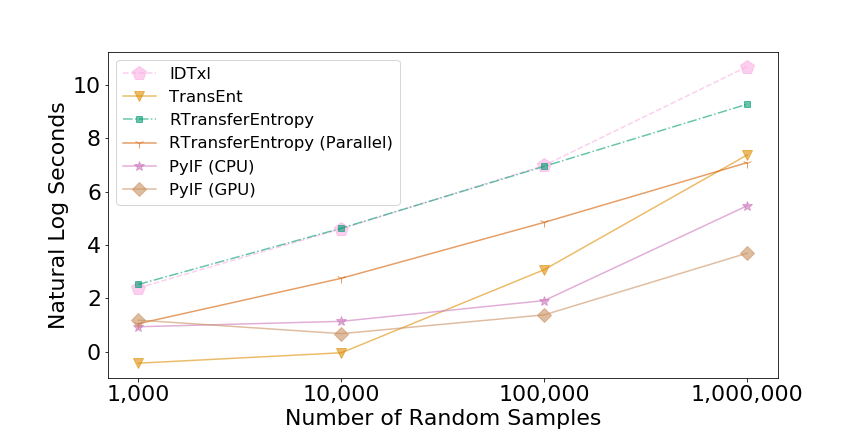
\includegraphics[scale=0.3]{figures/WallTime-TE.png}}
  \caption{This figure shows the natural log time( in seconds) to estimate Transfer Entropy for each implementation (excluding Transfer Entropy Toolbox) for each dataset used in this study. }
  \label{TE-walltime}
\end{figure}


\begin{figure}
  \centerline{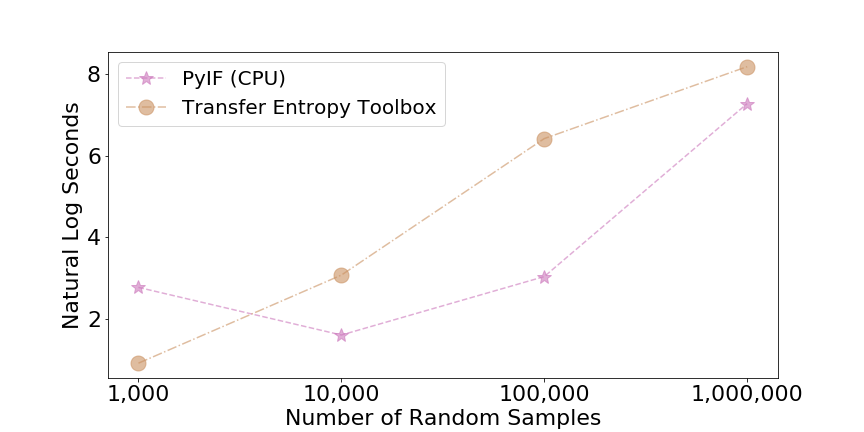
\includegraphics[scale=0.3]{figures/WallTime-TE2.png}}
  \caption{This figure shows the natural log time( in seconds) to estimate Transfer Entropy between PyIF and Transfer Entropy Toolbox on an Engineering Workstation as described in the section Comparative Analysis. Transfer Entropy Toolbox exceeded the maximum allowable CPU runtime for the Large Dataset. }
  \label{TE-walltime2}
\end{figure}


\begin{table}[htbp]
		\caption{The wall time to estimate Transfer Entropy for a variety of implementations on the different data sets described in the section Comparative Analysis.  The higher the wall time the longer it took for the implementation to estimate Transfer Entropy. The number in the relative performance indicates how many times faster (or slower) PyIF (CPU) is to a particular implementation. }
	\begin{center}
		\begin{tabular}{ |p{4cm}|p{1cm}| p{2cm}|  }
			\hline
			Implementation & Wall Time (in seconds) &  Relative Performance to PyIF (CPU)\\
 			\hline
			 \multicolumn{3}{|c|}{Micro Dataset Results (1000 Obs.)} \\
 			\hline
			IDTxl   & 10.98 & 4.28\\
 			TransEnt   & 0.656 & 0.25\\
	 		RTransferEntropy   & 12.492 & 4.87\\
	 		RTransferEntropy (Parallel) & 2.876 & 1.12\\
 			PyIF (CPU)   & 2.564 & 1.00\\
 			PyIF (GPU) & 3.282  & 1.28\\
 			 \hline
 			\multicolumn{3}{|c|}{Small Dataset Results (10,000 Obs.)} \\
 			\hline
		 	IDTxl   & 100.23 & 31.94\\
		 	TransEnt   & 0.968 & .308\\
 			RTransferEntropy   & 102.228 & 32.57\\
 			RTransferEntropy (Parallel) & 15.703 & 5.00\\
 			PyIF (CPU)   & 3.138 & 1.00\\
			 PyIF (GPU) & 1.98 & 0.63\\
 			 \hline
 			\multicolumn{3}{|c|}{Medium Dataset Results (100,000 Obs.)} \\
 			\hline
		 	IDTxl   & 1070.749 & 152.89\\
		 	TransEnt   & 21.708 & 3.03\\
 			RTransferEntropy   & 1036.661 & 152.00\\
 			RTransferEntropy (Parallel) & 127.281 & 18.66\\
 			PyIF (CPU)   & 6.82 & 1.00\\
			PyIF (GPU) & 3.996 & 0.58\\
 			 \hline
 			\multicolumn{3}{|c|}{Large Dataset Results (1,000,000 Obs.)} \\
 			\hline
		 	IDTxl   &  43150.129 & 181.97\\
		 	TransEnt   & 1585.942 & 6.68\\
 			RTransferEntropy   & 10592.77 & 44.67\\
 			RTransferEntropy (Parallel) & 1188.636 & 5.01\\
 			PyIF (CPU)   & 237.122 & 1.00\\
			 PyIF (GPU) & 40.231 & 0.16\\
			 \hline

		\end{tabular}
	\end{center}
	
		
	\label{DataTable}
\end{table}


\begin{table}[htbp]
	\caption{The wall time and relative performance to PyIF (CPU) to estimate Transfer Entropy between PyIF and Transfer Entropy Toolbox on an Engineering Workstation machine as described in the section Comparative Analysis.}
	\begin{center}
		\begin{tabular}{ |p{3cm}|p{2cm}| p{2cm}|  }
			\hline
			Implementation & Wall Time (in seconds) &  Relative Performance to PyIF (CPU) \\
 			\hline
			 \multicolumn{3}{|c|}{Micro Dataset Results (1000 Obs.)} \\
 			\hline
 			PyIF (CPU)   & 16.049 & 1.00\\
 			Transfer Entropy Toolbox & 2.5012 & 0.15 \\
 			 \hline
 			\multicolumn{3}{|c|}{Small Dataset Results (10,000 Obs.)} \\
 			\hline
 			PyIF (CPU)   & 4.989 & 1.00\\
			 Transfer Entropy Toolbox & 21.6880 & 4.347 \\
 			 \hline
 			\multicolumn{3}{|c|}{Medium Dataset Results (100,000 Obs.)} \\
 			\hline
 			PyIF (CPU)   & 20.915 & 1.00\\
			Transfer Entropy Toolbox & 616.8712 & 29.49 \\
 			 \hline
 			\multicolumn{3}{|c|}{Large Dataset Results (1,00,000 Obs.)} \\
 			\hline
 			PyIF (CPU)   & 1455.725 & 1.00\\
			 Transfer Entropy Toolbox & $>$ 3600 & $>$ 2.47\\
			 \hline
			 

		\end{tabular}
	\end{center}
	\label{DataTable-MATLAB}
	
\end{table}


\section{Conclusion}

An important issue is addressed regarding Big Data with respect to estimating bi-variate Transfer Entropy. We introduce a fast solution to estimate Transfer Entropy with a small amount of dependencies. On large data our implementation PyIF is up to 1072 times faster utilizing GPUs and up to 181 times faster utilizing CPUs than existing implementations that estimate bi-variate TE. PyIF is also open sourced and publicly available on github for anyone to use.  For future work we plan to improve the existing code base to increase the computation performance of PyIF even further. In addition to this we plan to implement additional estimators outlined in the section entitled "Estimating Transfer Entropy" to estimate bi-variate TE. This boost in computational performance will enable researchers to estimate bi-variate TE much faster for a variety of research applications. 

\section*{Acknowledgments}
This work was partially funded by the Graduate College Fellowship program at the University of Illinois. This work utilizes resources provided by the Innovative Systems Laboratory at the National Center for Supercomputing Applications at the University of Illinois at Urbana-Champaign. Lastly, we would like to thank Alice Perng for helpful work in Analysis 2.


\begin{thebibliography}{00}
\bibitem{InfoTheoryApplications} Stone, James V. Information Theory: A Tutorial Introduction. S.l.: Sebtel Press, 2015. Print.

\bibitem{IntroToTransferEntropy} Schreiber, Thomas. (2000). Measuring Information Transfer. Physical review letters. 85. 461-4. 10.1103/PhysRevLett.85.461.

\bibitem{IntroToTransferEntropy2} Palus, Milan \& Komarek, Vladimir \& Hrncír, Zbynek \& Sterbová, Katalin. (2001). Synchronization as adjustment of information rates: Detection from bivariate time series. Physical review. E, Statistical, nonlinear, and soft matter physics. 63. 046211. 10.1103/PhysRevE.63.046211.

\bibitem{FinAppTE} R. Marschinski and H. Kantz. Analysing the information flow between financial time series. The European Physical Journal B-Condensed Matter and Complex Systems, 30(2):275–281, 2002.

\bibitem{TEBook} Bossomaier, Terry, Lionel Barnett, Michael Harre, and Joseph T. Lizier. An Introduction to Transfer Entropy: Information Flow in Complex Systems. Cham: Springer, 2016. Internet resource.

\bibitem{MIdiffTE} A. Kaiser and T. Schreiber. Information transfer in continuous processes. Physica D, 166:43–62, 2002.

\bibitem{b359} P. L. Williams and R. D. Beer. Generalized measures of information transfer. 2011. arXiv:1102.1507.

\bibitem{kraskovEstimator} A. Kraskov, H. Stogbauer, and P. Grassberger. Estimating mutual information. Physical Review E, 69:066138–066153, 2004.

\bibitem{CUDA} Sanders, Jason, and Edward Kandrot. CUDA by example: an introduction to general-purpose GPU programming. Addison-Wesley Professional, 2010.

\bibitem{EstimatingTE} Khan, Shiraj \& Bandyopadhyay, Sharba \& Ganguly, Auroop \& Saigal, Sunil \& J Erickson, David \& Protopopescu, Vladimir \& Ostrouchov, George. (2007). Relative performance of mutual information estimation methods for quantifying the dependence among short and noisy data. Physical review. E, Statistical, nonlinear, and soft matter physics. 76. 026209. 10.1103/PhysRevE.76.026209.

\bibitem{KDE} Y. I. Moon, B. Rajagopalan, and U. Lall, Phys. Rev. E 52, 2318 1995.

\bibitem{NetworkTEApp1}  C. Damiani and P. Lecca. Model identification using correlation-based inference and transfer entropy estimation. In Proceedings of the 2011 Fifth UKSim European Symposium on
Computer Modeling and Simulation (EMS), pages 129–134. IEEE, 2011.

\bibitem{NetworkTEApp2} T. L. Bauer, R. Colbaugh, K. Glass, and D. Schnizlein. Use of transfer entropy to infer
relationships from behavior. In Proceedings of the Eighth Annual Cyber Security and Information Intelligence Research Workshop, CSIIRW ’13, New York, NY, USA, 2013. ACM.

\bibitem{NetworkTEApp3} C. J. Honey, R. Kotter, M. Breakspear, and O. Sporns. Network structure of cerebral cortex shapes functional connectivity on multiple time scales. Proceedings of the National Academy of Sciences of the United States of America, 104(24):10240–10245, 2007.

\bibitem{NetworkTEApp4} R. Vicente and M. Wibral. Efficient estimation of information transfer. In M. Wibral, R. Vicente, and J. T. Lizier, editors, Directed Information Measures in Neuroscience, Understanding Complex Systems, pages 37–58. Springer, Berlin/Heidelberg, 2014.

\bibitem{NetworkTEApp5} M. Wibral, R. Vicente, and M. Lindner. Transfer entropy in neuroscience. In M. Wibral, R. Vicente, and J. T. Lizier, editors, Directed Information Measures in Neuroscience, Understanding Complex Systems, pages 3–36. Springer, Berlin/Heidelberg, 2014

\bibitem{scipy} Jones, Eric, Travis Oliphant, and Pearu Peterson. "SciPy: Open source scientific tools for Python." (2001).

\bibitem{numpy} Developers, NumPy. "NumPy." NumPy Numpy. Scipy Developers (2013).

\bibitem{sklearn} Pedregosa, Fabian, et al. "Scikit-learn: Machine learning in Python." Journal of machine learning research 12.Oct (2011): 2825-2830.

\bibitem{nose} Pellerin, Jason. “Nose.” Nose 1.3.7 Documentation, https://nose.readthedocs.io/en/latest/.

\bibitem{numba} Lam, Siu Kwan, Antoine Pitrou, and Stanley Seibert. "Numba: A llvm-based python jit compiler." Proceedings of the Second Workshop on the LLVM Compiler Infrastructure in HPC. ACM, 2015.





\bibitem{IDTxl} Wollstadt, Patricia \& Lizier, Joseph \& Vicente, Raul \& Finn, Conor \& Martínez Zarzuela, Mario \& Mediano, Pedro \& Novelli, Leonardo \& Wibral, Michael. (2019). IDTxl: The Information Dynamics Toolkit xl: a Python package for the efficient analysis of multivariate information dynamics in networks. Journal of Open Source Software. 4. 1081. 10.21105/joss.01081.

\bibitem{TransEnt} ANN Library: David Mount, Sunil Arya. Transfer Entropy Packge:  Ghazaleh Haratinezhad Torbati and Glenn Lawyer. (2015).  TransferEntropy: The Transfer Entropy Package. R package version 1.5.  \url{https://CRAN.R-project.org/package=TransferEntropy}

\bibitem{ANN} Mount, D.M. ANN Programming Manual; Department of Computer Science, University of Maryland: College Park, MD, USA, 2006; pp. 4–25.

\bibitem{RTransferEntropy} Simon B, Thomas D, Franziska J. P, David J. Z (2019). “RTransferEntropy — Quantifying information flow between different time series using effective transfer entropy.” SoftwareX, 10(100265), 1-9. \url{https://doi.org/10.1016/j.softx.2019.100265}.

\bibitem{TransferEntropyToolbox} Lindner, Michael \& Vicente, Raul \& Priesemann, Viola \& Wibral, Michael. (2011). TRENTOOL: A MATLAB open source toolbox to analyse information flow in time series data with transfer entropy. BMC neuroscience. 12. 119. 10.1186/1471-2202-12-119.

\end{thebibliography}


\end{document}
